\documentclass[10pt,a4paper]{article}
\usepackage[margin=2.2cm]{geometry}
\usepackage[T1]{fontenc}
\usepackage[utf8]{inputenc}
\usepackage{lmodern}
\usepackage{amsmath,amssymb,bm}
\usepackage{graphicx}
\usepackage{booktabs}
\usepackage{xcolor}
\usepackage[authoryear,round]{natbib}
\usepackage[colorlinks=true,linkcolor=blue!50!black,citecolor=blue!50!black,urlcolor=blue!50!black]{hyperref}
\usepackage{caption}
\usepackage{subcaption}
\captionsetup{font=small,labelfont=bf}

% ---------------------------------------------------------------------------
% numbers, tables and figures are generated from the cached results of the code
% (paper/scripts/make_paper_assets.py); \pend marks a missing number
% ---------------------------------------------------------------------------
\newcommand{\pend}[1]{\textcolor{orange!80!black}{[#1]}}
% generated by paper/scripts/make_paper_assets.py -- do not edit
% source: qg2l_realism_sweep.ipynb @ cac38b6 (small size, before tuning / seeds)
\newcommand{\refmethod}{4DVar}
\newcommand{\kLyap}{192}
\newcommand{\stateDim}{2048}
\newcommand{\resultsSize}{small}
\expandafter\def\csname nu@Base\endcsname{73}
\expandafter\def\csname lam@Base\endcsname{0.093}
\expandafter\def\csname lamtau@Base\endcsname{0.98}
\expandafter\def\csname rev@Base\endcsname{10.5}
\expandafter\def\csname omt@Base\endcsname{0.60}
\expandafter\def\csname r@RD@Neu@Base\endcsname{1.07\,[1.03,\,1.11]}
\expandafter\def\csname rv@RD@Neu@Base\endcsname{1.07}
\expandafter\def\csname r@RD@Res@Base\endcsname{1.07\,[1.06,\,1.07]}
\expandafter\def\csname rv@RD@Res@Base\endcsname{1.07}
\expandafter\def\csname r@RD@Stab@Base\endcsname{1.13\,[1.08,\,1.17]}
\expandafter\def\csname rv@RD@Stab@Base\endcsname{1.13}
\expandafter\def\csname r@RD@Tot@Base\endcsname{1.09\,[1.08,\,1.11]}
\expandafter\def\csname rv@RD@Tot@Base\endcsname{1.09}
\expandafter\def\csname r@RD@Unst@Base\endcsname{1.15\,[1.09,\,1.21]}
\expandafter\def\csname rv@RD@Unst@Base\endcsname{1.15}
\expandafter\def\csname r@RO@Neu@Base\endcsname{0.99\,[0.98,\,1.00]}
\expandafter\def\csname rv@RO@Neu@Base\endcsname{0.99}
\expandafter\def\csname r@RO@Res@Base\endcsname{1.00\,[1.00,\,1.00]}
\expandafter\def\csname rv@RO@Res@Base\endcsname{1.00}
\expandafter\def\csname r@RO@Stab@Base\endcsname{1.00\,[1.00,\,1.01]}
\expandafter\def\csname rv@RO@Stab@Base\endcsname{1.00}
\expandafter\def\csname r@RO@Tot@Base\endcsname{1.00\,[0.99,\,1.01]}
\expandafter\def\csname rv@RO@Tot@Base\endcsname{1.00}
\expandafter\def\csname r@RO@Unst@Base\endcsname{1.00\,[0.98,\,1.01]}
\expandafter\def\csname rv@RO@Unst@Base\endcsname{1.00}
\expandafter\def\csname r@Net@Neu@Base\endcsname{1.50\,[1.23,\,1.85]}
\expandafter\def\csname rv@Net@Neu@Base\endcsname{1.50}
\expandafter\def\csname r@Net@Res@Base\endcsname{0.95\,[0.89,\,1.01]}
\expandafter\def\csname rv@Net@Res@Base\endcsname{0.95}
\expandafter\def\csname r@Net@Stab@Base\endcsname{1.23\,[1.04,\,1.44]}
\expandafter\def\csname rv@Net@Stab@Base\endcsname{1.23}
\expandafter\def\csname r@Net@Tot@Base\endcsname{1.24\,[1.15,\,1.34]}
\expandafter\def\csname rv@Net@Tot@Base\endcsname{1.24}
\expandafter\def\csname r@Net@Unst@Base\endcsname{3.39\,[2.93,\,3.87]}
\expandafter\def\csname rv@Net@Unst@Base\endcsname{3.39}
\expandafter\def\csname r@HybSeven@Neu@Base\endcsname{1.23\,[0.99,\,1.53]}
\expandafter\def\csname rv@HybSeven@Neu@Base\endcsname{1.23}
\expandafter\def\csname r@HybSeven@Res@Base\endcsname{1.13\,[1.08,\,1.19]}
\expandafter\def\csname rv@HybSeven@Res@Base\endcsname{1.13}
\expandafter\def\csname r@HybSeven@Stab@Base\endcsname{1.26\,[1.07,\,1.46]}
\expandafter\def\csname rv@HybSeven@Stab@Base\endcsname{1.26}
\expandafter\def\csname r@HybSeven@Tot@Base\endcsname{1.28\,[1.18,\,1.39]}
\expandafter\def\csname rv@HybSeven@Tot@Base\endcsname{1.28}
\expandafter\def\csname r@HybSeven@Unst@Base\endcsname{1.87\,[1.59,\,2.21]}
\expandafter\def\csname rv@HybSeven@Unst@Base\endcsname{1.87}
\expandafter\def\csname r@HybThree@Neu@Base\endcsname{1.44\,[1.15,\,1.80]}
\expandafter\def\csname rv@HybThree@Neu@Base\endcsname{1.44}
\expandafter\def\csname r@HybThree@Res@Base\endcsname{1.12\,[1.06,\,1.18]}
\expandafter\def\csname rv@HybThree@Res@Base\endcsname{1.12}
\expandafter\def\csname r@HybThree@Stab@Base\endcsname{1.25\,[1.06,\,1.47]}
\expandafter\def\csname rv@HybThree@Stab@Base\endcsname{1.25}
\expandafter\def\csname r@HybThree@Tot@Base\endcsname{1.35\,[1.24,\,1.46]}
\expandafter\def\csname rv@HybThree@Tot@Base\endcsname{1.35}
\expandafter\def\csname r@HybThree@Unst@Base\endcsname{2.64\,[2.28,\,3.04]}
\expandafter\def\csname rv@HybThree@Unst@Base\endcsname{2.64}
\expandafter\def\csname r@Hyb@Neu@Base\endcsname{1.50\,[1.20,\,1.87]}
\expandafter\def\csname rv@Hyb@Neu@Base\endcsname{1.50}
\expandafter\def\csname r@Hyb@Res@Base\endcsname{1.13\,[1.07,\,1.20]}
\expandafter\def\csname rv@Hyb@Res@Base\endcsname{1.13}
\expandafter\def\csname r@Hyb@Stab@Base\endcsname{1.28\,[1.10,\,1.48]}
\expandafter\def\csname rv@Hyb@Stab@Base\endcsname{1.28}
\expandafter\def\csname r@Hyb@Tot@Base\endcsname{1.38\,[1.28,\,1.50]}
\expandafter\def\csname rv@Hyb@Tot@Base\endcsname{1.38}
\expandafter\def\csname r@Hyb@Unst@Base\endcsname{2.88\,[2.51,\,3.32]}
\expandafter\def\csname rv@Hyb@Unst@Base\endcsname{2.88}
\expandafter\def\csname ssh@Net@Base\endcsname{0.51}
\expandafter\def\csname ltwo@Net@Base\endcsname{0.54}
\expandafter\def\csname lx@Net@Base\endcsname{51}
\expandafter\def\csname ssh@Var@Base\endcsname{0.90}
\expandafter\def\csname ltwo@Var@Base\endcsname{0.47}
\expandafter\def\csname lx@Var@Base\endcsname{60}
\expandafter\def\csname ssh@Weak@Base\endcsname{0.99}
\expandafter\def\csname ltwo@Weak@Base\endcsname{0.41}
\expandafter\def\csname lx@Weak@Base\endcsname{60}
\expandafter\def\csname ssh@Incr@Base\endcsname{0.85}
\expandafter\def\csname ltwo@Incr@Base\endcsname{0.45}
\expandafter\def\csname lx@Incr@Base\endcsname{59}
\expandafter\def\csname ssh@Budget@Base\endcsname{2.16}
\expandafter\def\csname ltwo@Budget@Base\endcsname{0.89}
\expandafter\def\csname lx@Budget@Base\endcsname{106}
\expandafter\def\csname ssh@RD@Base\endcsname{0.84}
\expandafter\def\csname ltwo@RD@Base\endcsname{0.42}
\expandafter\def\csname lx@RD@Base\endcsname{60}
\expandafter\def\csname ssh@RO@Base\endcsname{0.90}
\expandafter\def\csname ltwo@RO@Base\endcsname{0.47}
\expandafter\def\csname lx@RO@Base\endcsname{60}
\expandafter\def\csname ssh@HybSeven@Base\endcsname{0.68}
\expandafter\def\csname ltwo@HybSeven@Base\endcsname{0.49}
\expandafter\def\csname lx@HybSeven@Base\endcsname{54}
\expandafter\def\csname ssh@HybThree@Base\endcsname{0.62}
\expandafter\def\csname ltwo@HybThree@Base\endcsname{0.53}
\expandafter\def\csname lx@HybThree@Base\endcsname{51}
\expandafter\def\csname ssh@Hyb@Base\endcsname{0.57}
\expandafter\def\csname ltwo@Hyb@Base\endcsname{0.53}
\expandafter\def\csname lx@Hyb@Base\endcsname{51}
\expandafter\def\csname nu@ObsSig\endcsname{73}
\expandafter\def\csname lam@ObsSig\endcsname{0.093}
\expandafter\def\csname lamtau@ObsSig\endcsname{0.98}
\expandafter\def\csname rev@ObsSig\endcsname{10.5}
\expandafter\def\csname omt@ObsSig\endcsname{1.47}
\expandafter\def\csname r@RD@Neu@ObsSig\endcsname{1.32\,[1.22,\,1.41]}
\expandafter\def\csname rv@RD@Neu@ObsSig\endcsname{1.32}
\expandafter\def\csname r@RD@Res@ObsSig\endcsname{1.41\,[1.37,\,1.45]}
\expandafter\def\csname rv@RD@Res@ObsSig\endcsname{1.41}
\expandafter\def\csname r@RD@Stab@ObsSig\endcsname{1.56\,[1.50,\,1.63]}
\expandafter\def\csname rv@RD@Stab@ObsSig\endcsname{1.56}
\expandafter\def\csname r@RD@Tot@ObsSig\endcsname{1.39\,[1.33,\,1.44]}
\expandafter\def\csname rv@RD@Tot@ObsSig\endcsname{1.39}
\expandafter\def\csname r@RD@Unst@ObsSig\endcsname{1.32\,[1.20,\,1.43]}
\expandafter\def\csname rv@RD@Unst@ObsSig\endcsname{1.32}
\expandafter\def\csname r@RO@Neu@ObsSig\endcsname{1.32\,[1.21,\,1.42]}
\expandafter\def\csname rv@RO@Neu@ObsSig\endcsname{1.32}
\expandafter\def\csname r@RO@Res@ObsSig\endcsname{1.45\,[1.41,\,1.49]}
\expandafter\def\csname rv@RO@Res@ObsSig\endcsname{1.45}
\expandafter\def\csname r@RO@Stab@ObsSig\endcsname{1.59\,[1.52,\,1.66]}
\expandafter\def\csname rv@RO@Stab@ObsSig\endcsname{1.59}
\expandafter\def\csname r@RO@Tot@ObsSig\endcsname{1.42\,[1.37,\,1.47]}
\expandafter\def\csname rv@RO@Tot@ObsSig\endcsname{1.42}
\expandafter\def\csname r@RO@Unst@ObsSig\endcsname{1.34\,[1.24,\,1.46]}
\expandafter\def\csname rv@RO@Unst@ObsSig\endcsname{1.34}
\expandafter\def\csname r@Net@Neu@ObsSig\endcsname{2.30\,[2.14,\,2.46]}
\expandafter\def\csname rv@Net@Neu@ObsSig\endcsname{2.30}
\expandafter\def\csname r@Net@Res@ObsSig\endcsname{1.03\,[0.97,\,1.08]}
\expandafter\def\csname rv@Net@Res@ObsSig\endcsname{1.03}
\expandafter\def\csname r@Net@Stab@ObsSig\endcsname{1.73\,[1.53,\,1.96]}
\expandafter\def\csname rv@Net@Stab@ObsSig\endcsname{1.73}
\expandafter\def\csname r@Net@Tot@ObsSig\endcsname{1.67\,[1.58,\,1.76]}
\expandafter\def\csname rv@Net@Tot@ObsSig\endcsname{1.67}
\expandafter\def\csname r@Net@Unst@ObsSig\endcsname{5.25\,[4.80,\,5.72]}
\expandafter\def\csname rv@Net@Unst@ObsSig\endcsname{5.25}
\expandafter\def\csname r@HybSeven@Neu@ObsSig\endcsname{1.33\,[1.25,\,1.41]}
\expandafter\def\csname rv@HybSeven@Neu@ObsSig\endcsname{1.33}
\expandafter\def\csname r@HybSeven@Res@ObsSig\endcsname{1.26\,[1.20,\,1.32]}
\expandafter\def\csname rv@HybSeven@Res@ObsSig\endcsname{1.26}
\expandafter\def\csname r@HybSeven@Stab@ObsSig\endcsname{1.23\,[1.11,\,1.36]}
\expandafter\def\csname rv@HybSeven@Stab@ObsSig\endcsname{1.23}
\expandafter\def\csname r@HybSeven@Tot@ObsSig\endcsname{1.39\,[1.33,\,1.47]}
\expandafter\def\csname rv@HybSeven@Tot@ObsSig\endcsname{1.39}
\expandafter\def\csname r@HybSeven@Unst@ObsSig\endcsname{1.75\,[1.57,\,1.94]}
\expandafter\def\csname rv@HybSeven@Unst@ObsSig\endcsname{1.75}
\expandafter\def\csname r@HybThree@Neu@ObsSig\endcsname{1.49\,[1.43,\,1.57]}
\expandafter\def\csname rv@HybThree@Neu@ObsSig\endcsname{1.49}
\expandafter\def\csname r@HybThree@Res@ObsSig\endcsname{1.23\,[1.17,\,1.29]}
\expandafter\def\csname rv@HybThree@Res@ObsSig\endcsname{1.23}
\expandafter\def\csname r@HybThree@Stab@ObsSig\endcsname{1.34\,[1.19,\,1.50]}
\expandafter\def\csname rv@HybThree@Stab@ObsSig\endcsname{1.34}
\expandafter\def\csname r@HybThree@Tot@ObsSig\endcsname{1.53\,[1.45,\,1.61]}
\expandafter\def\csname rv@HybThree@Tot@ObsSig\endcsname{1.53}
\expandafter\def\csname r@HybThree@Unst@ObsSig\endcsname{2.40\,[2.17,\,2.61]}
\expandafter\def\csname rv@HybThree@Unst@ObsSig\endcsname{2.40}
\expandafter\def\csname r@Hyb@Neu@ObsSig\endcsname{1.90\,[1.82,\,2.00]}
\expandafter\def\csname rv@Hyb@Neu@ObsSig\endcsname{1.90}
\expandafter\def\csname r@Hyb@Res@ObsSig\endcsname{1.34\,[1.28,\,1.41]}
\expandafter\def\csname rv@Hyb@Res@ObsSig\endcsname{1.34}
\expandafter\def\csname r@Hyb@Stab@ObsSig\endcsname{1.55\,[1.36,\,1.77]}
\expandafter\def\csname rv@Hyb@Stab@ObsSig\endcsname{1.55}
\expandafter\def\csname r@Hyb@Tot@ObsSig\endcsname{1.80\,[1.70,\,1.89]}
\expandafter\def\csname rv@Hyb@Tot@ObsSig\endcsname{1.80}
\expandafter\def\csname r@Hyb@Unst@ObsSig\endcsname{3.42\,[3.08,\,3.73]}
\expandafter\def\csname rv@Hyb@Unst@ObsSig\endcsname{3.42}
\expandafter\def\csname ssh@Net@ObsSig\endcsname{0.79}
\expandafter\def\csname ltwo@Net@ObsSig\endcsname{0.61}
\expandafter\def\csname lx@Net@ObsSig\endcsname{61}
\expandafter\def\csname ssh@Var@ObsSig\endcsname{1.61}
\expandafter\def\csname ltwo@Var@ObsSig\endcsname{0.73}
\expandafter\def\csname lx@Var@ObsSig\endcsname{82}
\expandafter\def\csname ssh@Weak@ObsSig\endcsname{1.83}
\expandafter\def\csname ltwo@Weak@ObsSig\endcsname{0.73}
\expandafter\def\csname lx@Weak@ObsSig\endcsname{84}
\expandafter\def\csname ssh@Incr@ObsSig\endcsname{1.68}
\expandafter\def\csname ltwo@Incr@ObsSig\endcsname{0.77}
\expandafter\def\csname lx@Incr@ObsSig\endcsname{82}
\expandafter\def\csname ssh@Budget@ObsSig\endcsname{2.15}
\expandafter\def\csname ltwo@Budget@ObsSig\endcsname{0.84}
\expandafter\def\csname lx@Budget@ObsSig\endcsname{105}
\expandafter\def\csname ssh@HybSeven@ObsSig\endcsname{1.33}
\expandafter\def\csname ltwo@HybSeven@ObsSig\endcsname{0.60}
\expandafter\def\csname lx@HybSeven@ObsSig\endcsname{66}
\expandafter\def\csname ssh@RD@ObsSig\endcsname{1.36}
\expandafter\def\csname ltwo@RD@ObsSig\endcsname{0.54}
\expandafter\def\csname lx@RD@ObsSig\endcsname{74}
\expandafter\def\csname ssh@RO@ObsSig\endcsname{1.35}
\expandafter\def\csname ltwo@RO@ObsSig\endcsname{0.50}
\expandafter\def\csname lx@RO@ObsSig\endcsname{74}
\expandafter\def\csname ssh@HybThree@ObsSig\endcsname{1.25}
\expandafter\def\csname ltwo@HybThree@ObsSig\endcsname{0.65}
\expandafter\def\csname lx@HybThree@ObsSig\endcsname{61}
\expandafter\def\csname ssh@Hyb@ObsSig\endcsname{1.01}
\expandafter\def\csname ltwo@Hyb@ObsSig\endcsname{0.61}
\expandafter\def\csname lx@Hyb@ObsSig\endcsname{61}
\expandafter\def\csname nu@ParErr\endcsname{80}
\expandafter\def\csname lam@ParErr\endcsname{0.095}
\expandafter\def\csname lamtau@ParErr\endcsname{0.99}
\expandafter\def\csname rev@ParErr\endcsname{10.5}
\expandafter\def\csname omt@ParErr\endcsname{0.60}
\expandafter\def\csname r@RD@Neu@ParErr\endcsname{1.03\,[0.98,\,1.07]}
\expandafter\def\csname rv@RD@Neu@ParErr\endcsname{1.03}
\expandafter\def\csname r@RD@Res@ParErr\endcsname{1.05\,[1.03,\,1.07]}
\expandafter\def\csname rv@RD@Res@ParErr\endcsname{1.05}
\expandafter\def\csname r@RD@Stab@ParErr\endcsname{1.07\,[1.03,\,1.11]}
\expandafter\def\csname rv@RD@Stab@ParErr\endcsname{1.07}
\expandafter\def\csname r@RD@Tot@ParErr\endcsname{1.07\,[1.04,\,1.10]}
\expandafter\def\csname rv@RD@Tot@ParErr\endcsname{1.07}
\expandafter\def\csname r@RD@Unst@ParErr\endcsname{1.13\,[1.06,\,1.20]}
\expandafter\def\csname rv@RD@Unst@ParErr\endcsname{1.13}
\expandafter\def\csname r@RO@Neu@ParErr\endcsname{1.00\,[0.99,\,1.01]}
\expandafter\def\csname rv@RO@Neu@ParErr\endcsname{1.00}
\expandafter\def\csname r@RO@Res@ParErr\endcsname{1.00\,[1.00,\,1.00]}
\expandafter\def\csname rv@RO@Res@ParErr\endcsname{1.00}
\expandafter\def\csname r@RO@Stab@ParErr\endcsname{1.01\,[1.00,\,1.02]}
\expandafter\def\csname rv@RO@Stab@ParErr\endcsname{1.01}
\expandafter\def\csname r@RO@Tot@ParErr\endcsname{1.00\,[1.00,\,1.01]}
\expandafter\def\csname rv@RO@Tot@ParErr\endcsname{1.00}
\expandafter\def\csname r@RO@Unst@ParErr\endcsname{1.00\,[1.00,\,1.01]}
\expandafter\def\csname rv@RO@Unst@ParErr\endcsname{1.00}
\expandafter\def\csname r@Net@Neu@ParErr\endcsname{2.23\,[1.83,\,2.73]}
\expandafter\def\csname rv@Net@Neu@ParErr\endcsname{2.23}
\expandafter\def\csname r@Net@Res@ParErr\endcsname{1.16\,[1.10,\,1.21]}
\expandafter\def\csname rv@Net@Res@ParErr\endcsname{1.16}
\expandafter\def\csname r@Net@Stab@ParErr\endcsname{2.39\,[2.00,\,2.85]}
\expandafter\def\csname rv@Net@Stab@ParErr\endcsname{2.39}
\expandafter\def\csname r@Net@Tot@ParErr\endcsname{1.66\,[1.54,\,1.78]}
\expandafter\def\csname rv@Net@Tot@ParErr\endcsname{1.66}
\expandafter\def\csname r@Net@Unst@ParErr\endcsname{4.39\,[3.78,\,5.03]}
\expandafter\def\csname rv@Net@Unst@ParErr\endcsname{4.39}
\expandafter\def\csname r@HybSeven@Neu@ParErr\endcsname{1.89\,[1.63,\,2.20]}
\expandafter\def\csname rv@HybSeven@Neu@ParErr\endcsname{1.89}
\expandafter\def\csname r@HybSeven@Res@ParErr\endcsname{1.38\,[1.31,\,1.45]}
\expandafter\def\csname rv@HybSeven@Res@ParErr\endcsname{1.38}
\expandafter\def\csname r@HybSeven@Stab@ParErr\endcsname{2.30\,[2.01,\,2.60]}
\expandafter\def\csname rv@HybSeven@Stab@ParErr\endcsname{2.30}
\expandafter\def\csname r@HybSeven@Tot@ParErr\endcsname{1.68\,[1.57,\,1.80]}
\expandafter\def\csname rv@HybSeven@Tot@ParErr\endcsname{1.68}
\expandafter\def\csname r@HybSeven@Unst@ParErr\endcsname{2.25\,[1.92,\,2.59]}
\expandafter\def\csname rv@HybSeven@Unst@ParErr\endcsname{2.25}
\expandafter\def\csname r@HybThree@Neu@ParErr\endcsname{2.15\,[1.80,\,2.55]}
\expandafter\def\csname rv@HybThree@Neu@ParErr\endcsname{2.15}
\expandafter\def\csname r@HybThree@Res@ParErr\endcsname{1.39\,[1.32,\,1.46]}
\expandafter\def\csname rv@HybThree@Res@ParErr\endcsname{1.39}
\expandafter\def\csname r@HybThree@Stab@ParErr\endcsname{2.48\,[2.11,\,2.90]}
\expandafter\def\csname rv@HybThree@Stab@ParErr\endcsname{2.48}
\expandafter\def\csname r@HybThree@Tot@ParErr\endcsname{1.84\,[1.71,\,1.97]}
\expandafter\def\csname rv@HybThree@Tot@ParErr\endcsname{1.84}
\expandafter\def\csname r@HybThree@Unst@ParErr\endcsname{3.41\,[2.97,\,3.90]}
\expandafter\def\csname rv@HybThree@Unst@ParErr\endcsname{3.41}
\expandafter\def\csname r@Hyb@Neu@ParErr\endcsname{2.23\,[1.84,\,2.68]}
\expandafter\def\csname rv@Hyb@Neu@ParErr\endcsname{2.23}
\expandafter\def\csname r@Hyb@Res@ParErr\endcsname{1.41\,[1.34,\,1.48]}
\expandafter\def\csname rv@Hyb@Res@ParErr\endcsname{1.41}
\expandafter\def\csname r@Hyb@Stab@ParErr\endcsname{2.55\,[2.18,\,2.97]}
\expandafter\def\csname rv@Hyb@Stab@ParErr\endcsname{2.55}
\expandafter\def\csname r@Hyb@Tot@ParErr\endcsname{1.89\,[1.76,\,2.01]}
\expandafter\def\csname rv@Hyb@Tot@ParErr\endcsname{1.89}
\expandafter\def\csname r@Hyb@Unst@ParErr\endcsname{3.74\,[3.25,\,4.26]}
\expandafter\def\csname rv@Hyb@Unst@ParErr\endcsname{3.74}
\expandafter\def\csname ssh@Net@ParErr\endcsname{0.49}
\expandafter\def\csname ltwo@Net@ParErr\endcsname{0.42}
\expandafter\def\csname lx@Net@ParErr\endcsname{50}
\expandafter\def\csname ssh@Var@ParErr\endcsname{0.95}
\expandafter\def\csname ltwo@Var@ParErr\endcsname{0.56}
\expandafter\def\csname lx@Var@ParErr\endcsname{60}
\expandafter\def\csname ssh@Weak@ParErr\endcsname{1.03}
\expandafter\def\csname ltwo@Weak@ParErr\endcsname{0.54}
\expandafter\def\csname lx@Weak@ParErr\endcsname{60}
\expandafter\def\csname ssh@Incr@ParErr\endcsname{0.96}
\expandafter\def\csname ltwo@Incr@ParErr\endcsname{0.58}
\expandafter\def\csname lx@Incr@ParErr\endcsname{59}
\expandafter\def\csname ssh@Budget@ParErr\endcsname{2.09}
\expandafter\def\csname ltwo@Budget@ParErr\endcsname{0.82}
\expandafter\def\csname lx@Budget@ParErr\endcsname{103}
\expandafter\def\csname ssh@HybSeven@ParErr\endcsname{0.65}
\expandafter\def\csname ltwo@HybSeven@ParErr\endcsname{0.37}
\expandafter\def\csname lx@HybSeven@ParErr\endcsname{53}
\expandafter\def\csname ssh@RD@ParErr\endcsname{0.89}
\expandafter\def\csname ltwo@RD@ParErr\endcsname{0.55}
\expandafter\def\csname lx@RD@ParErr\endcsname{60}
\expandafter\def\csname ssh@RO@ParErr\endcsname{0.95}
\expandafter\def\csname ltwo@RO@ParErr\endcsname{0.56}
\expandafter\def\csname lx@RO@ParErr\endcsname{60}
\expandafter\def\csname ssh@HybThree@ParErr\endcsname{0.59}
\expandafter\def\csname ltwo@HybThree@ParErr\endcsname{0.41}
\expandafter\def\csname lx@HybThree@ParErr\endcsname{50}
\expandafter\def\csname ssh@Hyb@ParErr\endcsname{0.55}
\expandafter\def\csname ltwo@Hyb@ParErr\endcsname{0.40}
\expandafter\def\csname lx@Hyb@ParErr\endcsname{50}
\expandafter\def\csname nu@Bfree\endcsname{73}
\expandafter\def\csname lam@Bfree\endcsname{0.093}
\expandafter\def\csname lamtau@Bfree\endcsname{0.98}
\expandafter\def\csname rev@Bfree\endcsname{10.5}
\expandafter\def\csname omt@Bfree\endcsname{0.60}
\expandafter\def\csname r@RD@Neu@Bfree\endcsname{1.07\,[1.03,\,1.11]}
\expandafter\def\csname rv@RD@Neu@Bfree\endcsname{1.07}
\expandafter\def\csname r@RD@Res@Bfree\endcsname{1.06\,[1.05,\,1.07]}
\expandafter\def\csname rv@RD@Res@Bfree\endcsname{1.06}
\expandafter\def\csname r@RD@Stab@Bfree\endcsname{1.12\,[1.08,\,1.15]}
\expandafter\def\csname rv@RD@Stab@Bfree\endcsname{1.12}
\expandafter\def\csname r@RD@Tot@Bfree\endcsname{1.08\,[1.07,\,1.09]}
\expandafter\def\csname rv@RD@Tot@Bfree\endcsname{1.08}
\expandafter\def\csname r@RD@Unst@Bfree\endcsname{1.11\,[1.06,\,1.16]}
\expandafter\def\csname rv@RD@Unst@Bfree\endcsname{1.11}
\expandafter\def\csname r@RO@Neu@Bfree\endcsname{1.00\,[1.00,\,1.01]}
\expandafter\def\csname rv@RO@Neu@Bfree\endcsname{1.00}
\expandafter\def\csname r@RO@Res@Bfree\endcsname{1.00\,[1.00,\,1.00]}
\expandafter\def\csname rv@RO@Res@Bfree\endcsname{1.00}
\expandafter\def\csname r@RO@Stab@Bfree\endcsname{0.99\,[0.98,\,1.00]}
\expandafter\def\csname rv@RO@Stab@Bfree\endcsname{0.99}
\expandafter\def\csname r@RO@Tot@Bfree\endcsname{1.00\,[0.99,\,1.00]}
\expandafter\def\csname rv@RO@Tot@Bfree\endcsname{1.00}
\expandafter\def\csname r@RO@Unst@Bfree\endcsname{1.00\,[0.98,\,1.02]}
\expandafter\def\csname rv@RO@Unst@Bfree\endcsname{1.00}
\expandafter\def\csname r@Net@Neu@Bfree\endcsname{1.46\,[1.19,\,1.81]}
\expandafter\def\csname rv@Net@Neu@Bfree\endcsname{1.46}
\expandafter\def\csname r@Net@Res@Bfree\endcsname{0.93\,[0.87,\,0.98]}
\expandafter\def\csname rv@Net@Res@Bfree\endcsname{0.93}
\expandafter\def\csname r@Net@Stab@Bfree\endcsname{1.18\,[1.00,\,1.39]}
\expandafter\def\csname rv@Net@Stab@Bfree\endcsname{1.18}
\expandafter\def\csname r@Net@Tot@Bfree\endcsname{1.20\,[1.11,\,1.29]}
\expandafter\def\csname rv@Net@Tot@Bfree\endcsname{1.20}
\expandafter\def\csname r@Net@Unst@Bfree\endcsname{3.21\,[2.75,\,3.66]}
\expandafter\def\csname rv@Net@Unst@Bfree\endcsname{3.21}
\expandafter\def\csname r@HybSeven@Neu@Bfree\endcsname{1.21\,[0.98,\,1.51]}
\expandafter\def\csname rv@HybSeven@Neu@Bfree\endcsname{1.21}
\expandafter\def\csname r@HybSeven@Res@Bfree\endcsname{1.11\,[1.06,\,1.16]}
\expandafter\def\csname rv@HybSeven@Res@Bfree\endcsname{1.11}
\expandafter\def\csname r@HybSeven@Stab@Bfree\endcsname{1.21\,[1.04,\,1.42]}
\expandafter\def\csname rv@HybSeven@Stab@Bfree\endcsname{1.21}
\expandafter\def\csname r@HybSeven@Tot@Bfree\endcsname{1.24\,[1.15,\,1.35]}
\expandafter\def\csname rv@HybSeven@Tot@Bfree\endcsname{1.24}
\expandafter\def\csname r@HybSeven@Unst@Bfree\endcsname{1.79\,[1.52,\,2.12]}
\expandafter\def\csname rv@HybSeven@Unst@Bfree\endcsname{1.79}
\expandafter\def\csname r@HybThree@Neu@Bfree\endcsname{1.40\,[1.13,\,1.76]}
\expandafter\def\csname rv@HybThree@Neu@Bfree\endcsname{1.40}
\expandafter\def\csname r@HybThree@Res@Bfree\endcsname{1.10\,[1.03,\,1.16]}
\expandafter\def\csname rv@HybThree@Res@Bfree\endcsname{1.10}
\expandafter\def\csname r@HybThree@Stab@Bfree\endcsname{1.20\,[1.02,\,1.41]}
\expandafter\def\csname rv@HybThree@Stab@Bfree\endcsname{1.20}
\expandafter\def\csname r@HybThree@Tot@Bfree\endcsname{1.30\,[1.20,\,1.41]}
\expandafter\def\csname rv@HybThree@Tot@Bfree\endcsname{1.30}
\expandafter\def\csname r@HybThree@Unst@Bfree\endcsname{2.50\,[2.15,\,2.88]}
\expandafter\def\csname rv@HybThree@Unst@Bfree\endcsname{2.50}
\expandafter\def\csname r@Hyb@Neu@Bfree\endcsname{1.46\,[1.17,\,1.84]}
\expandafter\def\csname rv@Hyb@Neu@Bfree\endcsname{1.46}
\expandafter\def\csname r@Hyb@Res@Bfree\endcsname{1.11\,[1.05,\,1.17]}
\expandafter\def\csname rv@Hyb@Res@Bfree\endcsname{1.11}
\expandafter\def\csname r@Hyb@Stab@Bfree\endcsname{1.23\,[1.06,\,1.43]}
\expandafter\def\csname rv@Hyb@Stab@Bfree\endcsname{1.23}
\expandafter\def\csname r@Hyb@Tot@Bfree\endcsname{1.34\,[1.24,\,1.45]}
\expandafter\def\csname rv@Hyb@Tot@Bfree\endcsname{1.34}
\expandafter\def\csname r@Hyb@Unst@Bfree\endcsname{2.76\,[2.38,\,3.17]}
\expandafter\def\csname rv@Hyb@Unst@Bfree\endcsname{2.76}
\expandafter\def\csname ssh@Net@Bfree\endcsname{0.51}
\expandafter\def\csname ltwo@Net@Bfree\endcsname{0.54}
\expandafter\def\csname lx@Net@Bfree\endcsname{51}
\expandafter\def\csname ssh@Var@Bfree\endcsname{0.88}
\expandafter\def\csname ltwo@Var@Bfree\endcsname{0.46}
\expandafter\def\csname lx@Var@Bfree\endcsname{60}
\expandafter\def\csname ssh@Weak@Bfree\endcsname{0.96}
\expandafter\def\csname ltwo@Weak@Bfree\endcsname{0.40}
\expandafter\def\csname lx@Weak@Bfree\endcsname{59}
\expandafter\def\csname ssh@Incr@Bfree\endcsname{0.82}
\expandafter\def\csname ltwo@Incr@Bfree\endcsname{0.44}
\expandafter\def\csname lx@Incr@Bfree\endcsname{59}
\expandafter\def\csname ssh@Budget@Bfree\endcsname{2.26}
\expandafter\def\csname ltwo@Budget@Bfree\endcsname{0.91}
\expandafter\def\csname lx@Budget@Bfree\endcsname{107}
\expandafter\def\csname ssh@HybSeven@Bfree\endcsname{0.67}
\expandafter\def\csname ltwo@HybSeven@Bfree\endcsname{0.49}
\expandafter\def\csname lx@HybSeven@Bfree\endcsname{54}
\expandafter\def\csname ssh@RD@Bfree\endcsname{0.82}
\expandafter\def\csname ltwo@RD@Bfree\endcsname{0.42}
\expandafter\def\csname lx@RD@Bfree\endcsname{60}
\expandafter\def\csname ssh@RO@Bfree\endcsname{0.88}
\expandafter\def\csname ltwo@RO@Bfree\endcsname{0.46}
\expandafter\def\csname lx@RO@Bfree\endcsname{60}
\expandafter\def\csname ssh@HybThree@Bfree\endcsname{0.61}
\expandafter\def\csname ltwo@HybThree@Bfree\endcsname{0.53}
\expandafter\def\csname lx@HybThree@Bfree\endcsname{51}
\expandafter\def\csname ssh@Hyb@Bfree\endcsname{0.56}
\expandafter\def\csname ltwo@Hyb@Bfree\endcsname{0.52}
\expandafter\def\csname lx@Hyb@Bfree\endcsname{51}
\expandafter\def\csname nu@Real\endcsname{75}
\expandafter\def\csname lam@Real\endcsname{0.096}
\expandafter\def\csname lamtau@Real\endcsname{1.01}
\expandafter\def\csname rev@Real\endcsname{10.5}
\expandafter\def\csname omt@Real\endcsname{1.53}
\expandafter\def\csname r@RD@Neu@Real\endcsname{1.38\,[1.27,\,1.49]}
\expandafter\def\csname rv@RD@Neu@Real\endcsname{1.38}
\expandafter\def\csname r@RD@Res@Real\endcsname{1.37\,[1.31,\,1.43]}
\expandafter\def\csname rv@RD@Res@Real\endcsname{1.37}
\expandafter\def\csname r@RD@Stab@Real\endcsname{1.59\,[1.50,\,1.68]}
\expandafter\def\csname rv@RD@Stab@Real\endcsname{1.59}
\expandafter\def\csname r@RD@Tot@Real\endcsname{1.34\,[1.27,\,1.42]}
\expandafter\def\csname rv@RD@Tot@Real\endcsname{1.34}
\expandafter\def\csname r@RD@Unst@Real\endcsname{1.20\,[1.11,\,1.30]}
\expandafter\def\csname rv@RD@Unst@Real\endcsname{1.20}
\expandafter\def\csname r@RO@Neu@Real\endcsname{1.48\,[1.35,\,1.62]}
\expandafter\def\csname rv@RO@Neu@Real\endcsname{1.48}
\expandafter\def\csname r@RO@Res@Real\endcsname{1.43\,[1.35,\,1.52]}
\expandafter\def\csname rv@RO@Res@Real\endcsname{1.43}
\expandafter\def\csname r@RO@Stab@Real\endcsname{1.69\,[1.57,\,1.80]}
\expandafter\def\csname rv@RO@Stab@Real\endcsname{1.69}
\expandafter\def\csname r@RO@Tot@Real\endcsname{1.39\,[1.30,\,1.49]}
\expandafter\def\csname rv@RO@Tot@Real\endcsname{1.39}
\expandafter\def\csname r@RO@Unst@Real\endcsname{1.20\,[1.09,\,1.33]}
\expandafter\def\csname rv@RO@Unst@Real\endcsname{1.20}
\expandafter\def\csname r@Net@Neu@Real\endcsname{3.76\,[3.24,\,4.29]}
\expandafter\def\csname rv@Net@Neu@Real\endcsname{3.76}
\expandafter\def\csname r@Net@Res@Real\endcsname{1.32\,[1.24,\,1.40]}
\expandafter\def\csname rv@Net@Res@Real\endcsname{1.32}
\expandafter\def\csname r@Net@Stab@Real\endcsname{3.11\,[2.82,\,3.42]}
\expandafter\def\csname rv@Net@Stab@Real\endcsname{3.11}
\expandafter\def\csname r@Net@Tot@Real\endcsname{2.22\,[2.08,\,2.38]}
\expandafter\def\csname rv@Net@Tot@Real\endcsname{2.22}
\expandafter\def\csname r@Net@Unst@Real\endcsname{5.45\,[5.07,\,5.85]}
\expandafter\def\csname rv@Net@Unst@Real\endcsname{5.45}
\expandafter\def\csname r@HybSeven@Neu@Real\endcsname{2.41\,[2.09,\,2.72]}
\expandafter\def\csname rv@HybSeven@Neu@Real\endcsname{2.41}
\expandafter\def\csname r@HybSeven@Res@Real\endcsname{1.57\,[1.50,\,1.64]}
\expandafter\def\csname rv@HybSeven@Res@Real\endcsname{1.57}
\expandafter\def\csname r@HybSeven@Stab@Real\endcsname{2.25\,[2.06,\,2.45]}
\expandafter\def\csname rv@HybSeven@Stab@Real\endcsname{2.25}
\expandafter\def\csname r@HybSeven@Tot@Real\endcsname{1.77\,[1.68,\,1.87]}
\expandafter\def\csname rv@HybSeven@Tot@Real\endcsname{1.77}
\expandafter\def\csname r@HybSeven@Unst@Real\endcsname{1.68\,[1.54,\,1.85]}
\expandafter\def\csname rv@HybSeven@Unst@Real\endcsname{1.68}
\expandafter\def\csname r@HybThree@Neu@Real\endcsname{2.63\,[2.26,\,3.02]}
\expandafter\def\csname rv@HybThree@Neu@Real\endcsname{2.63}
\expandafter\def\csname r@HybThree@Res@Real\endcsname{1.53\,[1.44,\,1.63]}
\expandafter\def\csname rv@HybThree@Res@Real\endcsname{1.53}
\expandafter\def\csname r@HybThree@Stab@Real\endcsname{2.43\,[2.24,\,2.64]}
\expandafter\def\csname rv@HybThree@Stab@Real\endcsname{2.43}
\expandafter\def\csname r@HybThree@Tot@Real\endcsname{2.02\,[1.89,\,2.16]}
\expandafter\def\csname rv@HybThree@Tot@Real\endcsname{2.02}
\expandafter\def\csname r@HybThree@Unst@Real\endcsname{2.63\,[2.42,\,2.87]}
\expandafter\def\csname rv@HybThree@Unst@Real\endcsname{2.63}
\expandafter\def\csname r@Hyb@Neu@Real\endcsname{3.28\,[2.83,\,3.76]}
\expandafter\def\csname rv@Hyb@Neu@Real\endcsname{3.28}
\expandafter\def\csname r@Hyb@Res@Real\endcsname{1.67\,[1.58,\,1.77]}
\expandafter\def\csname rv@Hyb@Res@Real\endcsname{1.67}
\expandafter\def\csname r@Hyb@Stab@Real\endcsname{2.89\,[2.63,\,3.16]}
\expandafter\def\csname rv@Hyb@Stab@Real\endcsname{2.89}
\expandafter\def\csname r@Hyb@Tot@Real\endcsname{2.37\,[2.23,\,2.51]}
\expandafter\def\csname rv@Hyb@Tot@Real\endcsname{2.37}
\expandafter\def\csname r@Hyb@Unst@Real\endcsname{3.63\,[3.39,\,3.91]}
\expandafter\def\csname rv@Hyb@Unst@Real\endcsname{3.63}
\expandafter\def\csname ssh@Net@Real\endcsname{0.91}
\expandafter\def\csname ltwo@Net@Real\endcsname{0.57}
\expandafter\def\csname lx@Net@Real\endcsname{60}
\expandafter\def\csname ssh@Var@Real\endcsname{1.87}
\expandafter\def\csname ltwo@Var@Real\endcsname{1.05}
\expandafter\def\csname lx@Var@Real\endcsname{80}
\expandafter\def\csname ssh@Weak@Real\endcsname{2.00}
\expandafter\def\csname ltwo@Weak@Real\endcsname{0.85}
\expandafter\def\csname lx@Weak@Real\endcsname{80}
\expandafter\def\csname ssh@Incr@Real\endcsname{1.76}
\expandafter\def\csname ltwo@Incr@Real\endcsname{1.07}
\expandafter\def\csname lx@Incr@Real\endcsname{79}
\expandafter\def\csname ssh@Budget@Real\endcsname{2.70}
\expandafter\def\csname ltwo@Budget@Real\endcsname{1.08}
\expandafter\def\csname lx@Budget@Real\endcsname{116}
\expandafter\def\csname ssh@HybSeven@Real\endcsname{1.48}
\expandafter\def\csname ltwo@HybSeven@Real\endcsname{0.66}
\expandafter\def\csname lx@HybSeven@Real\endcsname{66}
\expandafter\def\csname ssh@RD@Real\endcsname{1.63}
\expandafter\def\csname ltwo@RD@Real\endcsname{0.82}
\expandafter\def\csname lx@RD@Real\endcsname{73}
\expandafter\def\csname ssh@RO@Real\endcsname{1.62}
\expandafter\def\csname ltwo@RO@Real\endcsname{0.75}
\expandafter\def\csname lx@RO@Real\endcsname{74}
\expandafter\def\csname ssh@HybThree@Real\endcsname{1.38}
\expandafter\def\csname ltwo@HybThree@Real\endcsname{0.67}
\expandafter\def\csname lx@HybThree@Real\endcsname{61}
\expandafter\def\csname ssh@Hyb@Real\endcsname{1.12}
\expandafter\def\csname ltwo@Hyb@Real\endcsname{0.60}
\expandafter\def\csname lx@Hyb@Real\endcsname{60}

\makeatletter
\newcommand{\getnum}[1]{\ifcsname #1\endcsname\csname #1\endcsname\else\pend{?}\fi}
\makeatother
% ratio E_ref / E_method with 90% CI:  \ratio{method}{subspace}{scenario}
\newcommand{\ratio}[3]{\getnum{r@#1@#2@#3}}
\newcommand{\ratiov}[3]{\getnum{rv@#1@#2@#3}}
\newcommand{\nunst}[1]{\getnum{nu@#1}}
\newcommand{\lamtau}[1]{\getnum{lamtau@#1}}
\newcommand{\ssh}[2]{\getnum{ssh@#1@#2}}
\newcommand{\ltwo}[2]{\getnum{ltwo@#1@#2}}
\newcommand{\omt}[1]{\getnum{omt@#1}}

\newcommand{\x}{\mathbf{x}}
\newcommand{\y}{\mathbf{y}}
\newcommand{\M}{\mathcal{M}}
\newcommand{\Hop}{\mathcal{H}}
\newcommand{\B}{\mathbf{B}}
\newcommand{\R}{\mathbf{R}}
\newcommand{\E}{\mathbb{E}}
\newcommand{\code}{\url{https://github.com/maxbeauchamp/4dvarnet-starter/tree/qg2l-lyapunov-diag}}

\title{\bfseries Where does end-to-end learned data assimilation win?\\
\large A Lyapunov-subspace analysis of 4DVarNet versus 4DVar in a chaotic two-layer quasi-geostrophic ocean}
\author{Maxime Beauchamp\\
\small CMCC Foundation, Italy \quad and \quad IMT Atlantique, France}
\date{}

\begin{document}
\maketitle

\begin{abstract}
End-to-end learned variational schemes such as 4DVarNet now outperform operational interpolation of satellite
altimetry, but \emph{why} they win against a well-specified 4DVar in a chaotic system remains mostly empirical.
We introduce an open, controllable testbed --- a two-layer quasi-geostrophic (QG) model observed by synthetic nadir
and SWOT altimetry --- and a mechanistic diagnostic that projects reconstruction errors onto the backward and covariant
Lyapunov vectors of the assimilation model. We compare 4DVarNet (three training seeds) with strong-, weak-constraint
and incremental 4DVar whose hyper-parameters are tuned on validation data and whose observation-error statistics are
estimated by the Desroziers diagnostic, in two domain sizes and across scenarios that progressively break the
assumptions favourable to 4DVar (perfect model, resolvable observations, known $\R$). We find that
(i)~the gain of 4DVarNet is concentrated in the \emph{unstable} subspace, where its error energy is
$2.5$--$5\times$ lower than that of the tuned 4DVar, with bootstrap intervals far from unity and a seed-to-seed
spread of a few percent, consistent with the theory that dynamically consistent estimators let their error grow along
the unstable manifold;
(ii)~this factor grows with realism and with domain size, and the only advantage of 4DVar --- on the most stable
directions and, with a perfect model, on the unobserved deep layer --- is found in the small domain; it vanishes in
the larger domain, where 4DVarNet is better in every subspace and halves the total error energy;
(iii)~a short-window 4DVar initialised by 4DVarNet recovers part of these stable directions, which pays off in the
small domain but not in the larger one. Code, notebooks and the scripts generating every number of this paper are
available.\footnote{\code}
\end{abstract}

% ===========================================================================
\section{Introduction}
% ===========================================================================
Variational data assimilation (4DVar) estimates the state of a geophysical system as the minimiser of a cost
combining a background term, an observation term and, in its weak-constraint form, a model-error term
\citep{carrassi2018data}. In chaotic systems its practical limits are well known: the cost function becomes
increasingly non-convex beyond a few Lyapunov times \citep{pires1996extending}, the background, observation and
model-error covariances $\B$, $\R$, $\mathbf{Q}$ are poorly known, and operational systems must solve the problem
with a few tens of tangent-linear and adjoint integrations \citep{courtier1994strategy}.
End-to-end learned schemes such as 4DVarNet \citep{fablet2021learning} keep the variational structure but learn the
prior and the solver from data; for sea surface height (SSH) mapping from nadir and wide-swath (SWOT) altimetry they
substantially improve upon optimal interpolation \citep{beauchamp2023ssh,morrow2019global}.

Two arguments are usually put forward for this success. Statistically, a network trained with a mean-squared error
approximates the posterior mean $\E[\x\,|\,\y]$ under the training distribution, i.e.\ the Bayes estimator for
that loss, whereas 4DVar computes a maximum a posteriori estimate under Gaussian assumptions with hand-specified
statistics. Numerically, the learned solver performs amortised optimisation and can avoid the local minima of the
4DVar cost. Neither argument says \emph{which components of the error} are reduced, nor whether a carefully tuned
4DVar would close the gap. This paper answers these questions with the tools of the theory of assimilation in the
unstable subspace \citep{carrassi2007adaptive,trevisan2010four,bocquet2017degenerate}.

\paragraph{Contributions.}
\begin{itemize}\itemsep0pt
\item An open two-layer QG testbed with synthetic nadir + SWOT altimetry in which model error (resolution, physical
  parameters, unknown forcing), observation error (representativeness, unresolved signal, correlated SWOT errors) and
  background statistics can be switched on independently (Sec.~\ref{sec:testbed}).
\item A mechanistic diagnostic: projection of reconstruction errors onto the backward (BLV) and covariant (CLV)
  Lyapunov vectors of the assimilation model in the energy norm, with paired block-bootstrap confidence intervals
  (Sec.~\ref{sec:diag}).
\item A systematic comparison of 4DVarNet with nonlinear, incremental and low-budget 4DVar, including
  observation-error statistics estimated by the Desroziers diagnostic and hyper-parameters tuned on validation data,
  across realism scenarios and two domain sizes, with training-seed replicates (Sec.~\ref{sec:results}).
\item The finding that the gain of 4DVarNet lies in the unstable subspace and is robust to training seeds, realism
  and domain size, whereas the advantage of 4DVar is confined to the most stable directions of the small
  domain; a short-window hybrid exploits it only there.
\end{itemize}

% ===========================================================================
\section{Background}
% ===========================================================================
\paragraph{4DVar and 4DVarNet.}
Over a window $[t_0,t_T]$ with dynamics $\x_{t+1}=\M(\x_t)$ and observations $\y_t=\Hop_t(\x_t)+\bm{\varepsilon}_t$,
strong-constraint 4DVar minimises
\begin{equation}
J(\x_0)=\tfrac12\|\x_0-\x_b\|^2_{\B^{-1}}+\tfrac12\textstyle\sum_t\|\y_t-\Hop_t(\M_{0\to t}(\x_0))\|^2_{\R^{-1}} ,
\label{eq:4dvar}
\end{equation}
and the weak-constraint version adds $\tfrac12\sum_t\|\bm{\eta}_t\|^2_{\mathbf{Q}^{-1}}$ with
$\x_{t+1}=\M(\x_t)+\bm{\eta}_{t+1}$. With the control-variable transform $\x_0=\x_b+\B^{1/2}\mathbf{v}$ the
background Hessian becomes the identity; incremental 4DVar then alternates Gauss--Newton re-linearisations (outer
loops) and conjugate-gradient minimisations of the resulting quadratic cost (inner loops) using tangent-linear (TL)
and adjoint models \citep{courtier1994strategy}.
4DVarNet \citep{fablet2021learning} replaces the cost by $U_\Phi(\x,\y)=\|\y-\Hop(\x)\|^2_\Omega+\lambda\|\x-\Phi(\x)\|^2$
with a learned prior $\Phi$ (here a bilinear convolutional auto-encoder on the space-time state) and minimises it with
a learned gradient solver $\Gamma$ (ConvLSTM) unrolled for $K$ steps; $\Phi$ and $\Gamma$ are trained end-to-end with
a supervised reconstruction loss.

\paragraph{Lyapunov vectors and the unstable subspace.}
Let $\mathbf{M}_n$ be the tangent-linear propagator along a trajectory. The QR iteration
$\mathbf{M}_n\mathbf{V}_n=\mathbf{V}_{n+1}\mathbf{R}_{n+1}$ \citep{benettin1980lyapunov} yields the Lyapunov
exponents $\lambda_i$ (time averages of $\log|[\mathbf{R}_n]_{ii}|$) and the orthonormal backward Lyapunov vectors
$\mathbf{V}_n$; a backward iteration with $\mathbf{R}_n^{-1}$ gives the covariant Lyapunov vectors (CLV) spanning the
same nested subspaces \citep{ginelli2007characterizing}. The unstable-neutral subspace has dimension
$n_0=\#\{\lambda_i\ge0\}$. For linear(ised) filters and smoothers with deterministic dynamics, the error covariance
asymptotically collapses onto this subspace \citep{gurumoorthy2017rank,bocquet2017degenerate}, which motivates
assimilation in the unstable subspace \citep{trevisan2010four} and explains why ensembles of size $\gtrsim n_0$
suffice \citep{bocquet2017fourdenvar}. \emph{Corollary used here:} a dynamically consistent estimate (a model
trajectory, as in strong-constraint 4DVar) has an error whose unstable component grows within the window, while its
stable components are damped for free by the dynamics. A learned smoother is not constrained to be a model
trajectory; where its error lies in the Lyapunov spectrum is therefore an empirical question, which we answer.
Figure~\ref{fig:concept} illustrates these notions on Lorenz-63 and summarises the diagnostic and the mechanism
tested in this paper.

\begin{figure}[t]\centering
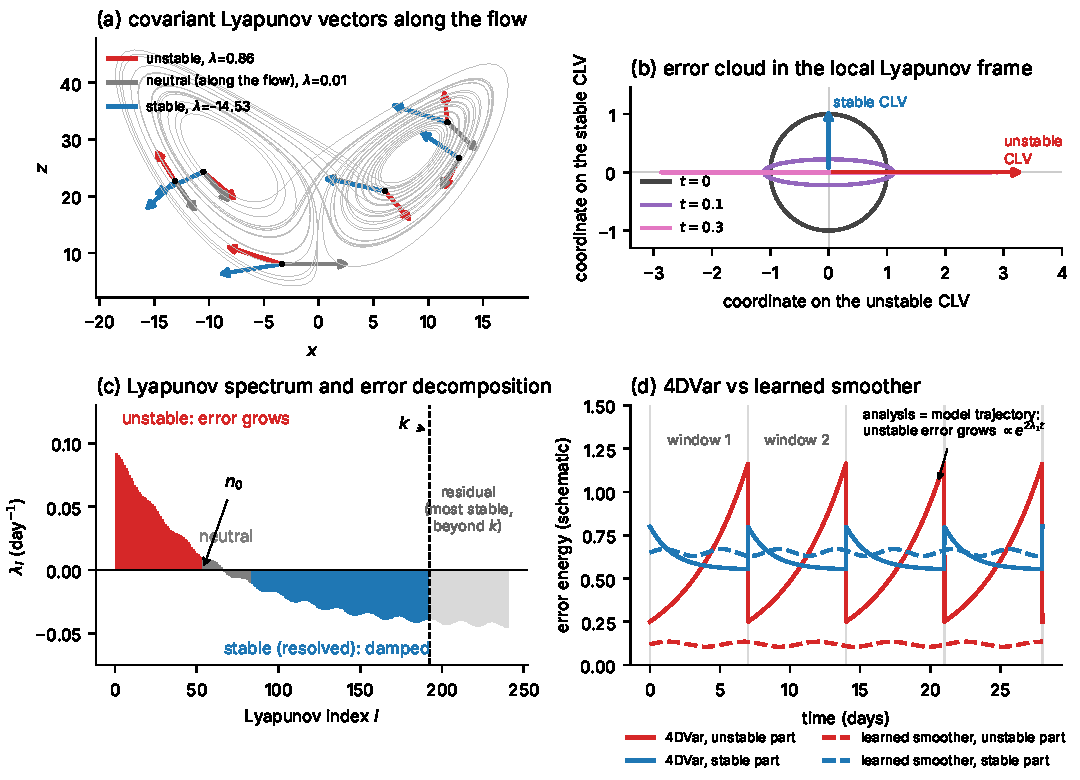
\includegraphics[width=\linewidth]{figures/concept.pdf}
\caption{Conceptual view. (a) Covariant Lyapunov vectors of Lorenz-63 along the attractor (Ginelli algorithm):
unstable (red), neutral, along the flow (grey), and stable (blue) directions, with their exponents.
(b) Tangent-linear evolution of a circle of initial errors, expressed in the local CLV frame: the error is
stretched along the unstable direction and collapses along the stable one, so that it ends up aligned with the
unstable subspace. (c) In a large chaotic system (here the spectrum of a QG-like model), the error of an estimate is
decomposed on the $n_0$ unstable, the neutral and the stable directions resolved by the $k$ computed vectors, plus a
residual on the most stable ones. (d) Mechanism examined in this paper (schematic): a dynamically consistent
estimate (strong-constraint 4DVar) is a model trajectory, so its unstable error grows within each window and is
reset by the observations of the next one, while the dynamics damps its stable error; a learned space-time smoother
is not a trajectory and is not subject to this growth.}
\label{fig:concept}
\end{figure}

% ===========================================================================
\section{Testbed}\label{sec:testbed}
% ===========================================================================
\paragraph{Model.} We use a two-layer QG model on a doubly periodic $\beta$-plane \citep{vallis2017atmospheric},
$\partial_t q_i+J(\psi_i,q_i)=\mathcal{D}_i$, $q_i=\nabla^2\psi_i+F_i(\psi_j-\psi_i)+\beta y$, with a background
shear driving baroclinic instability, bottom Ekman friction and a spectral filter (pseudo-spectral, RK4, numpy/torch
backends). Two domain sizes are used: a \emph{small} 500\,km box (truth at $64^2$, assimilation grid $32^2$) for the full
set of scenarios and methods, and a \emph{full} 1000\,km box (truth at $128^2$, assimilation grid $64^2$) for the
baseline and realistic scenarios; in both, $\Delta x=15.6$\,km and $R_d=15$\,km, and the high-resolution truth is
spectrally truncated to the assimilation grid: the low-resolution assimilation model has
a genuine, structured model error. SSH is $f_0\psi_1/g$; the deep layer is never observed. The flow is turbulent,
with SSH standard deviation $\approx7$\,cm and eddies of 100--200\,km (Fig.~\ref{fig:testbed}).

\paragraph{Observations.} Jason-3, Sentinel-3A/B (nadir, 1--1.4\,cm noise) and SWOT (two 50\,km KaRIn swaths around
a 20\,km nadir gap, 3\,mm noise) are simulated with their inclinations, repeat cycles and interleaved sub-cycles, with
the real ground-track spacing. The median revisit time is $\tau_{\mathrm{obs}}=\getnum{rev@Base}$\,days in the small box
and \getnum{rev@BaseFull}\,days in the full one, and the leading exponent of the assimilation model is
$\lambda_1\approx\getnum{lam@Base}$\,day$^{-1}$, so $\lambda_1\tau_{\mathrm{obs}}\approx\lamtau{Base}$ (resp.\
\lamtau{BaseFull}): the intermediate regime where neither dynamics nor statistics alone suffice.

\paragraph{Scenarios.} Starting from this \emph{baseline} (a favourable case for 4DVar: same equations, parameters
and forcing for truth and model, observations of resolvable scales with white noise of known variance, $\B$ estimated
from the truth), we break the assumptions one at a time (Table~\ref{tab:scen}). Each scenario has its own truth and
observations; 4DVarNet is retrained on each.

\begin{figure}[t]\centering
\begin{subfigure}[b]{0.205\linewidth}\centering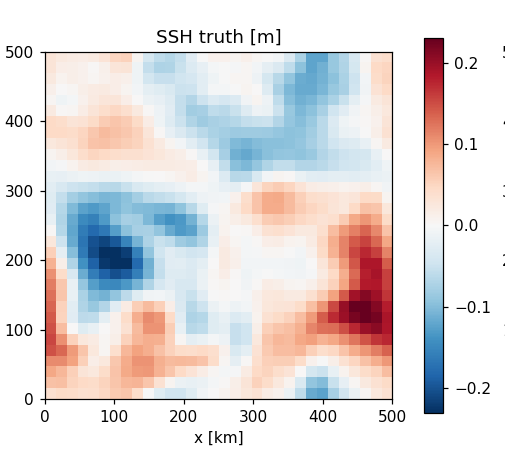
\includegraphics[height=3.0cm]{figures/testbed_truth_obs.png}
\caption{SSH truth}\end{subfigure}\hfill
\begin{subfigure}[b]{0.39\linewidth}\centering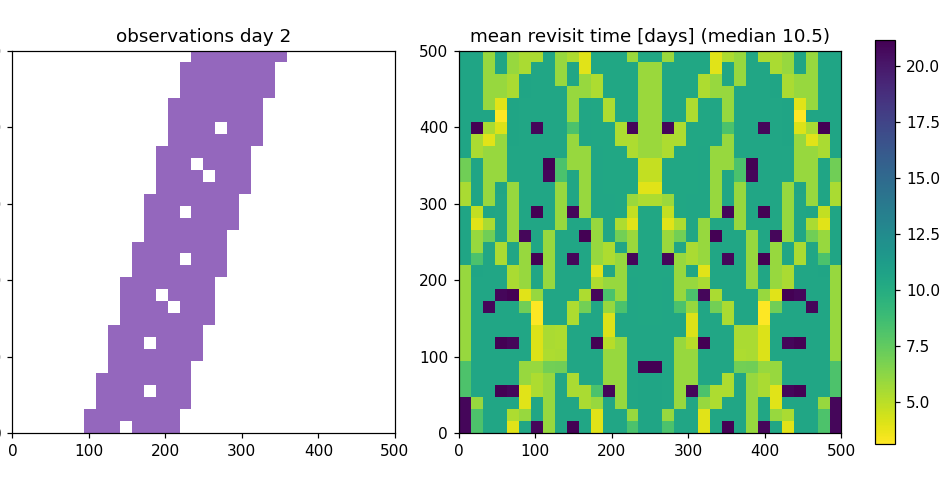
\includegraphics[height=3.0cm]{figures/testbed_swot_revisit.png}
\caption{SWOT pass, revisit time (days)}\end{subfigure}\hfill
\begin{subfigure}[b]{0.38\linewidth}\centering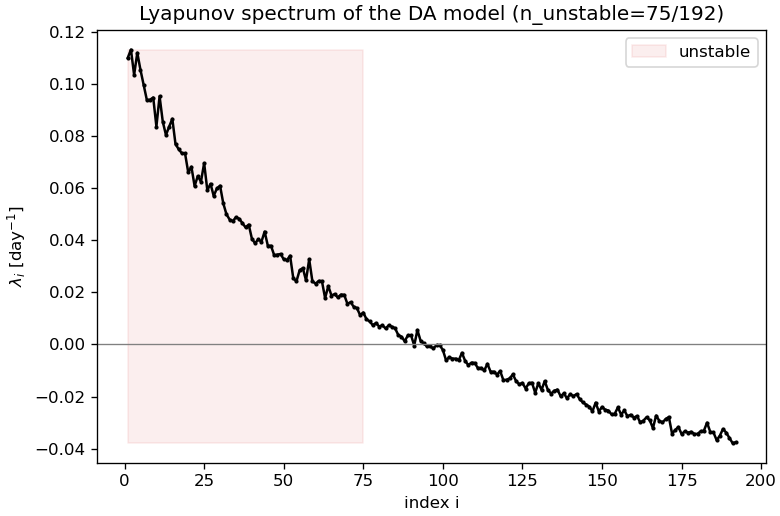
\includegraphics[height=3.0cm]{figures/lyapunov_spectrum.png}
\caption{Lyapunov spectrum}\end{subfigure}
\caption{Testbed (small configuration). (c) Lyapunov exponents of the assimilation model along the true trajectory
(realistic scenario, $k=\kLyap$ vectors): the spectrum is flat (extensive chaos), with
$n_0\approx\nunst{Real}$ unstable directions out of $\stateDim$.}
\label{fig:testbed}
\end{figure}

\begin{table}[t]\centering\small
\caption{Realism scenarios (each breaks one assumption favourable to 4DVar; \emph{realistic} combines them).}
\label{tab:scen}
\begin{tabular}{p{2.6cm}p{8.6cm}p{3.6cm}}\toprule
scenario & change & assumption broken\\\midrule
baseline & resolution only (high-resolution truth truncated to the model grid) & --- \\
free-run $\B$ & 4DVar $\B$ from a free run of the model instead of the truth & oracle $\B$ \\
unresolved signal & obs sample the block-averaged high-resolution SSH plus an internal-tide-like signal
(1\,cm, 40--120\,km, 1-day decorrelation) & resolvable obs, known $\R$ \\
parameter error & truth with bottom drag $\times1.5$ and $\beta\times0.8$ & perfect model \\
realistic & all of the above $+$ unknown stochastic forcing (2\,mm\,day$^{-1}$, 150--400\,km) and SWOT roll-like
correlated error (1\,cm per 100\,km) & all \\\bottomrule
\end{tabular}
\end{table}

\paragraph{Methods.} \emph{4DVarNet}: state $(\psi_1,\psi_2)$ in SSH-equivalent units over 21-day windows
(2--3 revisit times), observations on layer 1 only, circular padding, $K=15$ solver steps, trained on 3 years,
validated on 90 days, tested on 90 days with overlapping windows blended in time; three training seeds in the
baseline and realistic scenarios.
\emph{4DVar}: cycled windows, nonlinear low-resolution QG model, adjoint by automatic differentiation, homogeneous
isotropic two-layer spectral $\B$ (control-variable transform), diagonal $\R$.
Variants: L-BFGS on the preconditioned cost (near convergence; 7-day windows, $\approx1$ Lyapunov time, for the
untuned version); incremental Gauss--Newton/CG with $3\times20$ (operational-like) or $1\times5$ (low budget)
iterations; weak constraint (daily model-error forcing); $\R$ nominal, estimated by the Desroziers diagnostic
$\E[\mathbf{d}_a\mathbf{d}_b^\top]=\R$ on the validation period \citep{desroziers2005diagnosis} ($\R_{\mathrm D}$, no
truth used), or oracle. The \emph{tuned} 4DVar --- the reference of all ratios below --- selects the $\B$ scaling, the
window length and $\mathbf{Q}$ by a grid search on the validation period, the counterpart of 4DVarNet's training and
early stopping; it retains 10-day windows and $\B$ scalings of 0.25--1 depending on the scenario.
\emph{Hybrid}: incremental 4DVar with $\R_{\mathrm D}$ over 3-day windows whose background is the 4DVarNet
reconstruction.

% ===========================================================================
\section{Lyapunov-subspace error diagnostic}\label{sec:diag}
% ===========================================================================
Along the true trajectory we compute $k$ leading BLVs/CLVs of the daily flow map of the assimilation model, with a
central finite-difference TL model and orthonormality in the energy norm $\|\mathbf{e}\|^2_E=\|\mathbf{S}\mathbf{e}\|^2$,
$\mathbf{S}$ mapping $(\psi_1,\psi_2)$ to the kinetic and available potential energy fields. For each method and test
day, the error $\mathbf{e}=\hat\x-\x^{\mathrm{true}}$ (both layers) is decomposed orthogonally,
\begin{equation}
\|\mathbf{e}\|^2_E=\underbrace{\textstyle\sum_{\lambda_i>\epsilon}c_i^2}_{\text{unstable}}
+\underbrace{\textstyle\sum_{|\lambda_i|\le\epsilon}c_i^2}_{\text{neutral}}
+\underbrace{\textstyle\sum_{\lambda_i<-\epsilon,\,i\le k}c_i^2}_{\text{stable (resolved)}}
+\underbrace{\|\mathbf{e}-\mathbf{V}\mathbf{c}\|^2_E}_{\text{residual}},
\qquad c_i=\langle\mathbf{e},\mathbf{v}_i\rangle_E ,
\end{equation}
with $\epsilon=0.01$\,day$^{-1}$ and $k>n_0$, so that the residual collects the most stable directions. Oblique CLV
decompositions are ill-conditioned: the smallest principal angle between the unstable and stable CLV subspaces is
only $8$--$10^\circ$ here (near-tangencies), so we report orthogonal projections on the CLV subspaces instead.
Confidence intervals on the ratios $E_{\mathrm{ref}}/E_{\mathrm{method}}$ come from a paired moving-block bootstrap
(10-day blocks, $\approx1$ Lyapunov time, the same blocks for all methods). The forward and backward sweeps are
validated on Lorenz-96 (exponents, CLV covariance $\mathbf{M}_n\mathbf{c}_{i,n}\parallel\mathbf{c}_{i,n+1}$).

% ===========================================================================
\section{Results}\label{sec:results}
% ===========================================================================
\paragraph{Regime.} The spectrum is flat (Fig.~\ref{fig:testbed}c): $n_0\approx\nunst{Base}$ of $\stateDim$
directions are unstable in the small box and $\nunst{BaseFull}$ of $\stateDimFull$ in the full box ($\approx3.6\%$ in
both), i.e.\ the unstable dimension scales with the number of eddies, unlike Lorenz-96
\citep{lorenz1996predictability}. Low-rank arguments therefore hold relative to $n_0$, not in absolute dimension.

\begin{table}[t]\centering\small
\caption{Test RMSE (cm) of SSH (observed) and of the deep layer (never observed, SSH-equivalent); 4DVarNet: mean
($\pm$ s.d.) over three training seeds where available. Best in bold.}\label{tab:scores}
\textbf{(a) small domain} (500\,km, $32^2$)\\[2pt]
\resizebox{\linewidth}{!}{% generated by paper/scripts/make_paper_assets.py -- do not edit
\begin{tabular}{lcccccccc}
\toprule
 & \multicolumn{2}{c}{baseline} & \multicolumn{2}{c}{unresolved signal} & \multicolumn{2}{c}{parameter error} & \multicolumn{2}{c}{realistic} \\
\cmidrule(lr){2-3} \cmidrule(lr){4-5} \cmidrule(lr){6-7} \cmidrule(lr){8-9}
 & SSH & layer 2 & SSH & layer 2 & SSH & layer 2 & SSH & layer 2 \\
\midrule
4DVarNet & \textbf{0.51} & 0.54 & \textbf{0.79} & 0.61 & \textbf{0.49} & 0.42 & \textbf{0.91} & \textbf{0.57} \\
4DVar & 0.90 & 0.47 & 1.61 & 0.73 & 0.95 & 0.56 & 1.87 & 1.05 \\
4DVar, $\mathbf{R}_{\mathrm{D}}$ & 0.84 & \textbf{0.42} & 1.36 & \textbf{0.54} & 0.89 & 0.55 & 1.63 & 0.82 \\
4DVar incr.\ $3{\times}20$ & 0.85 & 0.45 & 1.68 & 0.77 & 0.96 & 0.58 & 1.76 & 1.07 \\
4DVar incr.\ $1{\times}5$ & 2.16 & 0.89 & 2.15 & 0.84 & 2.09 & 0.82 & 2.70 & 1.08 \\
Hybrid (3\,d, $\mathbf{R}_{\mathrm{D}}$) & 0.57 & 0.53 & 1.01 & 0.61 & 0.55 & \textbf{0.40} & 1.12 & 0.60 \\
\bottomrule
\end{tabular}
}\\[6pt]
\textbf{(b) full domain} (1000\,km, $64^2$)\\[2pt]
% generated by paper/scripts/make_paper_assets.py -- do not edit
\begin{tabular}{lcccc}
\toprule
 & \multicolumn{2}{c}{baseline} & \multicolumn{2}{c}{realistic} \\
\cmidrule(lr){2-3} \cmidrule(lr){4-5}
 & SSH & layer 2 & SSH & layer 2 \\
\midrule
4DVarNet & \textbf{0.48\,{\scriptsize($\pm$0.01)}} & 0.33\,{\scriptsize($\pm$0.01)} & \textbf{0.77} & \textbf{0.42} \\
4DVar, tuned & 0.95 & 0.44 & 1.48 & 0.76 \\
4DVar, untuned & 1.02 & 0.47 & 1.63 & 0.82 \\
4DVar incr.\ $3{\times}20$ & 1.00 & 0.49 & 1.65 & 0.90 \\
4DVar incr.\ $1{\times}5$ & 3.23 & 1.41 & 3.18 & 1.27 \\
Hybrid (3\,d) & 0.54 & \textbf{0.33} & 0.99 & 0.46 \\
\bottomrule
\end{tabular}

\end{table}

\paragraph{Scores.} On the observed variable 4DVarNet is the most accurate in every scenario and both domains
(Table~\ref{tab:scores}): \ssh{Net}{Base} vs \ssh{Tuned}{Base}\,cm for the tuned 4DVar in the small baseline,
\ssh{Net}{Real} vs \ssh{Tuned}{Real}\,cm in the small realistic scenario, and \ssh{Net}{BaseFull} vs
\ssh{Tuned}{BaseFull}, resp.\ \ssh{Net}{RealFull} vs \ssh{Tuned}{RealFull}\,cm in the full domain. On the unobserved
deep layer the picture depends on the configuration. In the small domain with a perfect model, 4DVar, which infers
$\psi_2$ through the exact baroclinic coupling, is better (baseline \ltwo{Tuned}{Base} vs \ltwo{Net}{Base}\,cm,
unresolved signal \ltwo{Tuned}{ObsSig} vs \ltwo{Net}{ObsSig}\,cm); under parameter error, in the realistic scenario
and in the full domain 4DVarNet is better (full baseline \ltwo{Net}{BaseFull} vs \ltwo{Tuned}{BaseFull}\,cm, full
realistic \ltwo{Net}{RealFull} vs \ltwo{Tuned}{RealFull}\,cm). Tuning matters: relative to the untuned 4DVar it
reduces the total error energy by a factor \getnum{rv@Tuned@Tot@Base@vsVar} (small baseline) to
\getnum{rv@Tuned@Tot@Real@vsVar} (small realistic), so that all comparisons below are against a 4DVar given the same
access to validation data as 4DVarNet. The incremental solver at $3\times20$ matches the nonlinear L-BFGS
minimisation, but a properly preconditioned 4DVar with $1\times5$ iterations collapses (\ssh{Budget}{Base}\,cm small,
\ssh{Budget}{BaseFull}\,cm full): the Hessian has as many eigenvalues $\gg1$ as there are directions constrained by the
precise SWOT data, far more than 5 CG iterations can capture, and analysis errors propagate through the cycled
background. Matching 4DVar requires $\sim10^3$ model integrations per 90 test days (Table~\ref{tab:cost}).

\begin{figure}[t]\centering
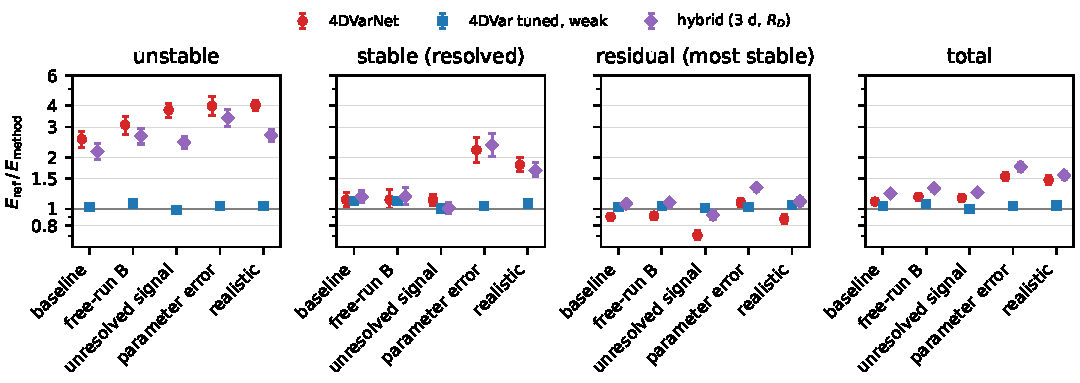
\includegraphics[width=\linewidth]{figures/ratios.pdf}
\caption{Error-energy ratio $E_{\mathrm{ref}}/E_{\mathrm{method}}$ per Lyapunov subspace (reference: \refmethod;
$>1$: the method is better), with 90\% paired block-bootstrap intervals; small dots: individual 4DVarNet training
seeds. Left of the dotted line: small domain, all scenarios; right: full domain.}
\label{fig:ratios}
\end{figure}

\paragraph{Where the gain lies.} Figure~\ref{fig:ratios} is the central result. In every scenario and both domains
the error energy of 4DVarNet is $2.5$--$5\times$ smaller than that of the tuned 4DVar in the \emph{unstable}
subspace (small domain: baseline \ratio{Net}{Unst}{Base}, unresolved signal \ratio{Net}{Unst}{ObsSig}, parameter
error \ratio{Net}{Unst}{ParErr}, realistic \ratio{Net}{Unst}{Real}; full domain: baseline \ratio{Net}{Unst}{BaseFull},
realistic \ratio{Net}{Unst}{RealFull}), with intervals far from 1; the factor grows with realism and with domain size.
The 4DVar error is aligned with the unstable manifold: it grows along the leading BLVs within each window (saw-tooth
in time), as predicted for dynamically consistent estimators, whereas the learned smoother is not a model trajectory
and does not let these directions grow. The untuned 4DVar loses mostly in the same subspace
(\ratiov{Var}{Unst}{Base}--\ratiov{Var}{Unst}{ParErr} relative to the tuned one), i.e.\ tuning narrows but does not
close the gap.

The advantage of 4DVar, where it exists, lies at the other end of the spectrum. In the small domain it is better in
the residual, most stable directions (baseline \ratio{Net}{Res}{Base}, unresolved signal
\ratio{Net}{Res}{ObsSig}, realistic \ratio{Net}{Res}{Real}), i.e.\ in the directions that its exact dynamics damps for
free. Under parameter error alone this advantage disappears (stable \ratio{Net}{Stab}{ParErr}, residual
\ratio{Net}{Res}{ParErr}), and in the full domain 4DVarNet is better in \emph{all} subspaces (stable resolved
\ratio{Net}{Stab}{BaseFull}, residual \ratio{Net}{Res}{BaseFull} in the baseline; \ratio{Net}{Stab}{RealFull} and
\ratio{Net}{Res}{RealFull} in the realistic scenario), so that its total error energy is about half that of the tuned
4DVar (\ratio{Net}{Tot}{BaseFull}, \ratio{Net}{Tot}{RealFull}). The full domain differs from the small one by a
shorter revisit time ($\lambda_1\tau_{\mathrm{obs}}\approx\lamtau{BaseFull}$ vs \lamtau{Base}) and by four times
more eddies per training window; our experiments do not separate the two effects, but both favour the learned prior
on the poorly observed, slowly varying directions.

\begin{table}[t]\centering\small
\caption{Robustness of 4DVarNet to the training seed: mean $\pm$ standard deviation over seeds of the SSH RMSE and of
the error-energy ratios to \refmethod.}\label{tab:seeds}
% generated -- do not edit
\pend{seed-to-seed variability: pending (sweep in progress)}

\end{table}

\paragraph{Robustness.} The seed-to-seed spread is small compared with the effects discussed
(Table~\ref{tab:seeds}): a few percent on the unstable ratio (e.g.\ $5.02\pm0.14$ in the full baseline) and on the
total, i.e.\ the conclusions are not an artefact of a lucky training run. The bootstrap intervals, which account for
the temporal correlation of the errors over one Lyapunov time, are of the same order. The source of $\B$ (truth vs
model free run) has no measurable effect in this homogeneous flow (\ratio{Net}{Tot}{Bfree} vs
\ratio{Net}{Tot}{Base}).

\paragraph{Observation-error statistics.} With an unresolved signal in the observations the actual observation error
rises from \omt{Base} to \omt{ObsSig}\,cm while the nominal $\R$ keeps the instrumental noise. The Desroziers
diagnostic recovers most of it without the truth (SWOT: \getnum{rdswot@ObsSig}\,cm vs \getnum{roswot@ObsSig}\,cm
actual), the spatially correlated part being under-estimated, and improves the untuned 4DVar by a factor
\getnum{rv@RD@Tot@ObsSig@vsVar} in total error energy. It brings 4DVar to within a few percent of the tuned
configuration (\ratio{RD}{Tot}{ObsSig}), and in the full baseline the tuning selects exactly the
$\R_{\mathrm D}$ configuration. Even so, 4DVarNet remains \ratiov{Net}{Unst}{ObsSig}$\times$ better in the unstable
subspace: a better $\R$ does not remove the within-window growth.

\paragraph{Hybrid.} Initialising a short (3-day) 4DVar with 4DVarNet and $\R_{\mathrm D}$ trades part of the unstable
gain (\ratio{Hyb}{Unst}{Base} vs \ratio{Net}{Unst}{Base} for 4DVarNet, small baseline) for the most stable directions
(\ratio{Hyb}{Res}{Base} vs \ratio{Net}{Res}{Base}). In the small domain, where 4DVarNet is weak on the latter, this
lowers the total error energy (baseline \ratio{Hyb}{Tot}{Base} vs \ratio{Net}{Tot}{Base}, realistic
\ratio{Hyb}{Tot}{Real} vs \ratio{Net}{Tot}{Real}). In the full domain there is little left to gain on the stable side
and the hybrid is on par with or behind 4DVarNet (baseline \ratio{Hyb}{Tot}{BaseFull} vs \ratio{Net}{Tot}{BaseFull},
realistic \ratio{Hyb}{Tot}{RealFull} vs \ratio{Net}{Tot}{RealFull}). On the observed SSH 4DVarNet alone is always
the most accurate (e.g.\ \ssh{Hyb}{RealFull} vs \ssh{Net}{RealFull}\,cm, full realistic). The hybrid costs about two
thirds of a tuned 4DVar (Table~\ref{tab:cost}).

\begin{table}[t]\centering\small
\caption{Model integrations over a 90-day test period (+ 30-day spin-up), small domain. 4DVarNet needs none at
inference (one forward pass of the network per window).}\label{tab:cost}
% generated -- do not edit
\begin{tabular}{lrrrr}
\toprule
method & nonlinear & tangent linear & adjoint & total \\
\midrule
4DVar, tuned ($\mathbf{R}_{\mathrm{D}}$) & 526 & 0 & 526 & 1052 \\
4DVar & 789 & 0 & 789 & 1578 \\
4DVar, $\mathbf{R}_{\mathrm{D}}$ & 787 & 0 & 787 & 1574 \\
4DVar incr.\ $3{\times}20$ & 72 & 1080 & 1134 & 2286 \\
4DVar incr.\ $1{\times}5$ & 36 & 90 & 108 & 234 \\
Hybrid (3\,d, $\mathbf{R}_{\mathrm{D}}$) & 60 & 300 & 330 & 690 \\
\bottomrule
\end{tabular}

\end{table}

% ===========================================================================
\section{Discussion and conclusion}
% ===========================================================================
The Lyapunov view turns the empirical superiority of 4DVarNet into a mechanism. A strong-constraint 4DVar returns a
model trajectory; between observations its error grows along the unstable directions and, by the classical collapse
results, is dominated by them, while the stable part is controlled for free by the dynamics. The learned
space-time smoother is not constrained to be a trajectory and is trained to minimise the expected error under the
actual sampling: it suppresses the growing directions $2.5$--$5\times$ better than a tuned 4DVar, robustly across
scenarios, training seeds and domain sizes. The dynamical consistency of 4DVar buys it an advantage only on the most
stable directions, and only in the small domain (on the deep layer, only with a perfect model); it disappears in the
larger domain, where 4DVarNet is better in every subspace and halves the total error energy. A short-window hybrid
exploits this complementarity where it exists, in the small domain, but brings nothing at the larger scale. For
practice, this suggests that the relevant question is not whether a learned scheme beats 4DVar on average, but whether
the dynamics of the assimilation model is accurate enough on the stable directions to be worth enforcing.

\emph{Limitations.} The testbed is periodic and quasi-geostrophic (no coasts, topography or internal tides); each
scenario uses one truth realisation (temporal bootstrap only), the full domain covers two scenarios, and seed
replicates are limited to three; the diagnostic uses the Lyapunov vectors of the assimilation model along the true
trajectory. Separating the effects of revisit time and training-sample size on the stable directions requires
dedicated experiments. \emph{Perspectives}: penalising the learned reconstruction in the stable subspace (dynamical
consistency losses), hybrid schemes with a learned background-error covariance, and the same diagnostic on SWOT
observing-system experiments.

\paragraph{Code and reproducibility.} Model, observation simulator, 4DVarNet, 4DVar (nonlinear, incremental,
weak-constraint, Desroziers, tuning), Lyapunov diagnostic, notebooks, Slurm scripts and the script generating all
tables, figures and numbers of this paper: \code.

\bibliographystyle{abbrvnat}
\bibliography{refs}
\end{document}
